% Written by ../code/make_numbers.py. Do not edit by hand.
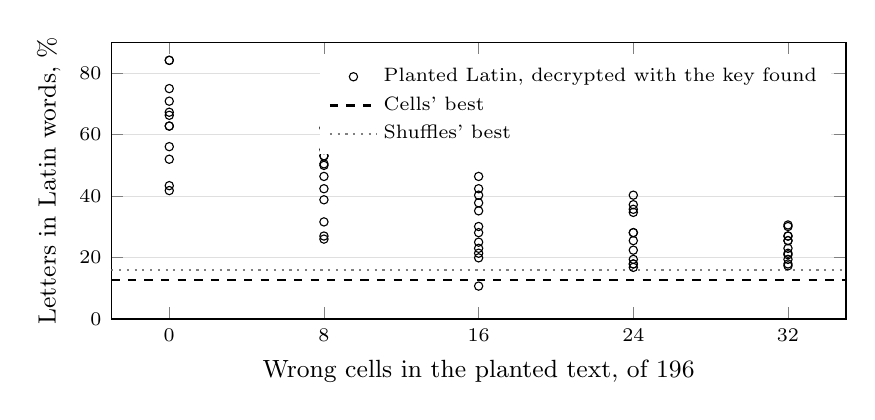
\begin{tikzpicture}
\begin{axis}[width=0.9\linewidth, height=0.42\linewidth,
  xmin=-3, xmax=35, ymin=0, ymax=90, xtick={0,8,16,24,32},
  xlabel={Wrong cells in the planted text, of 196}, ylabel={Letters in Latin words, \%},
  label style={font=\small}, ticklabel style={font=\scriptsize}, ymajorgrids, grid style={gray!25},
  legend style={font=\scriptsize, draw=none, at={(0.98,0.95)}, anchor=north east}, legend cell align=left]
\addplot[only marks, mark=o, mark size=1.5pt, black] coordinates {(0,41.8) (0,43.4) (0,52.0) (0,56.1) (0,62.8) (0,62.8) (0,66.3) (0,67.3) (0,70.9) (0,75.0) (0,84.2) (0,84.2) (8,26.0) (8,27.0) (8,31.6) (8,38.8) (8,42.4) (8,46.4) (8,50.0) (8,50.5) (8,53.1) (8,53.1) (8,55.1) (8,62.2) (16,10.7) (16,19.9) (16,21.4) (16,23.0) (16,25.0) (16,28.1) (16,30.1) (16,35.2) (16,37.8) (16,40.3) (16,42.4) (16,46.4) (24,16.8) (24,17.9) (24,17.9) (24,19.4) (24,22.4) (24,25.5) (24,28.1) (24,28.1) (24,34.7) (24,35.7) (24,37.2) (24,40.3) (32,17.3) (32,17.9) (32,19.4) (32,20.9) (32,21.4) (32,23.0) (32,25.5) (32,25.5) (32,27.0) (32,27.0) (32,30.1) (32,30.6)};
\addlegendentry{Planted Latin, decrypted with the key found}
\addplot[dashed, thick, black] coordinates {(-3,12.8) (35,12.8)};
\addlegendentry{Cells' best}
\addplot[dotted, thick, gray] coordinates {(-3,16.0) (35,16.0)};
\addlegendentry{Shuffles' best}
\end{axis}
\end{tikzpicture}
